\documentclass{article}
\usepackage{blindtext}
\usepackage{xcolor}
\usepackage{amsfonts}
\usepackage{hyperref} 
\usepackage{indentfirst}
\usepackage{graphicx}
\usepackage[normalem]{ulem}
\usepackage [english]{babel}
\usepackage [autostyle, english = american]{csquotes}
\usepackage{appendix}
\usepackage{tabularx}
\usepackage{bbm}
\usepackage{amsmath,amssymb}
\usepackage{mathtools}
\usepackage{makecell}
\graphicspath{ {./images/} }
\usepackage{enumitem}
\usepackage{soul}
\usepackage{mathtools}
\usepackage{wrapfig}
\usepackage{mathrsfs}
\usepackage{centernot}
\usepackage{amsthm}
%\bibliography{bibliograph}
%\usepackage{biblatex}

\allowdisplaybreaks

\MakeOuterQuote{"}

\newtheorem{theorem}{Theorem}[section]
\newtheorem{definition}[theorem]{Definition}
\newtheorem{corollary}[theorem]{Corollary}
\newtheorem{lemma}[theorem]{Lemma}
\newtheorem{proposition}[theorem]{Proposition}
\newtheorem{example}[theorem]{Example}
\newenvironment{remark}[1][Remark:]{\begin{trivlist}
		\item[\hskip \labelsep {\bfseries #1}]}{\end{trivlist}}

\newcommand{\defeq}{\mathrel{\mathop:}=}
\newcommand{\stackeq}[1]{\stackrel{\mathclap{\normalfont\mbox{\normalfont\tiny {#1}}}}{=}}
\newcommand\reals{\mathbb{R}}
\newcommand\field{\mathbb{F}}
\newcommand\complex{\mathbb{C}}
\newcommand\schwartz{\mathcal{S}}
\newcommand\naturals{\mathbb{N}}
\usepackage[a4paper,
bindingoffset=0.2in,
left=1in,
right=1in,
top=1in,
bottom=1in,
footskip=.25in]{geometry}
\hypersetup{
	colorlinks=false
}
%\setcounter{section}{-1}
\title{}
\author{Yung Chi Li\\ Advised by Maksym Radziwi\l\l}
%\date{January 2024}

\begin{document}
	\maketitle
	\begin{abstract}
		 
	\end{abstract}
	\section*{Notation}
Below are the notational preferences of the author.
\begin{enumerate}
    \item $p$ always denotes a prime, and by extension $p_j,p_n$ etc.
\end{enumerate}
	\section{Introduction to the Riemann Zeta Function}
We give a quick introduction to the Zeta function in this section, including its product representation and analytic continuation.
\begin{definition}[Zeta Function]
	Let $s\in\complex$ with $\Re(s)>1$. Then \begin{equation}
	\zeta(s)=\sum_{n=1}^{\infty}\frac{1}{n^s}.
	\end{equation}
\end{definition}
The zeta function converges absolutely on $\Re(s)>1$ by comparing to the integral $\int x^{-\Re(s)} dx$.
The properties of the zeta function as they relate to the distribution primes. In particular, the Dirichlet series can be represented as a product of primes.
\begin{proposition}\label{eulerproduct}
	On $\Re(s)>1$, \begin{equation}
		\zeta(s) = \prod_{p\in\mathbb{N}}\left(1-\frac{1}{p^s}\right)^{-1}.	
	\end{equation}
\end{proposition}
\begin{remark}
	This expresion also converges absolutely for $\Re(s)>1$. Since \[
		\left(1-\frac{1}{p^s}\right)^{-1} = \frac{p^s}{p^s-1} = 1 + \frac{1}{p^s-1}
	\]
	and $\sum(p^s-1)^{-1}$ converges absolutely by comparison to the zeta function Dirichlet series.
\end{remark}
\begin{proof}[Sketch of proof]
	Write $s=\sigma+it$. For each $p$,\[
		\left(1-\frac{1}{p^s}\right)^{-1} = \left(\frac{1}{p^s}+\frac{1}{p^{2s}}+\frac{1}{p^{3s}}+...\right)
	\]
	converges absolutely for $\Re(s)>1$ and uniformly across all $p$. We thus take for $m>N$ \begin{align*}
		\prod_{p\leq N}\left(1-\frac{1}{p^s}\right)^{-1}  &= \prod_{p\leq N}\left(\sum_{k=1}^{m} \frac{1}{p^{ks}}+O(2^{-m\sigma})\right)\\
		&\stackeq{(*)}\sum_{n=1}^{N}\frac{1}{n^s}+O_1(\sum_{n=N+1}^{\infty} \frac{1}{n^\sigma}) + O(2^{-m\sigma})\\
		&=\zeta(s) + O_1(\sum_{n=N+1}^{\infty} \frac{1}{n^\sigma}) + O(2^{-m\sigma})
	\end{align*}
	Where we apply to Fundemental Theorem of Arithmetic in (*) to show that each term $n^{-s}$ has coefficient $1$ determined by the unique prime factorization.
	As $m\to\infty$, $2^{-m\sigma} \to 0$. Then we take $N\to\infty$, the tail of the infinite sum converges to zero too.
\end{proof}
\begin{proposition} \label{analyticcontinuation}
	$\zeta$ extends to a meromorphic function on $\complex$ with a simple pole at $s=1$. By abuse of notation, we identify the extension of the zeta function with $\zeta$ too.
\end{proposition}

We will prove Proposition \ref{analyticcontinuation} in two steps. First, we will extend $\zeta$ to $\sigma>0$. Then, we will describe the continuation of the zeta function to the whole plane using by its functional equation: $\zeta$ has a line of symmetry across $\Re (s)=1/2$.
\begin{proposition}\label{extension}
	Let $\xi(s)\defeq \pi^{-s/2}\Gamma(s/2)\zeta(s)$. Then \begin{equation}\label{symmetryeq}
		\xi(s) = \xi(1-s).
	\end{equation}
\end{proposition}
\begin{proof}[Extension of $\zeta$ to $\sigma>0$]
	We apply integration by parts on Dirichlet series when $\sigma>1$ \begin{align*}
		\zeta(s)&=\int_{1/2}^{\infty} x^{-s} d \lfloor x \rfloor \\
				&= s \int_{1/2}^{\infty} \lfloor x \rfloor x^{-s-1} d x\\
				&=  s \int_{1}^{\infty}  x^{-s} - \frac{\{x\}}{x^{-s-1}} d x\\
				&= \frac{s}{s-1} - s \int_{1}^{\infty} \frac{\{x\}}{x^{-s-1}} dx\\
	\end{align*}
	where in the last expression, the integral converges when $\sigma>0$, and the pole at $s=1$ arises from the first term.
\end{proof}


\begin{proof}[Proof of Proposition \ref{extension}]
	Using \begin{align*}
		\Gamma(s)=\int_{0}^{\infty} e^{-x}x^{s-1}dx,
	\end{align*}
	we make the substitution $x=\pi n^2y$ to get \begin{align*}
		\Gamma(s)&= \int_{0}^{\infty} e^{-\pi n^2 y} (\pi n^2 y)^{s-1} \pi n^2 dy\\
		\implies \frac{\Gamma(s)}{\pi^s n^{2s}} &= \int_{0}^{\infty} e^{-\pi n^2 y} y^{s-1} dy
	\end{align*}
	So that by the Monotone Convergence Theorem,\begin{align*}
		\pi^{-s/2}\Gamma(s/2)\zeta(s) &= \sum_{n=1}^{\infty}\frac{\Gamma(s/2)}{\pi^{s/2} n^s}\\
		&= \sum_{n=1}^{\infty} \int_{0}^{\infty} e^{-\pi n^2x} x^{s/2-1} dx\\
		&=  \int_{0}^{\infty}\sum_{n=1}^{\infty}\left(e^{-\pi n^2 x}\right)  x^{s/2-1} dx.
	\end{align*}
	We now let \[
		\omega(x) = \sum_{n=1}^{\infty} e^{-\pi n^2 x}, \quad \theta(x) = \sum_{n=-\infty}^{\infty} e^{-\pi n^2 x} = 2\omega(x)+1,
	\]
	and apply Poisson Summation to \begin{align*}
		\theta(x) &= \sum_{n=-\infty}^{\infty} e^{-\pi n^2 x}\\
		&= \sum_{k=-\infty}^{\infty} \int_{-\infty}^{\infty} e^{-\pi y^2 x} e^{-2\pi i k y} dy\\
		&= \sum_{k=-\infty}^{\infty} \int_{-\infty}^{\infty} e^{-\pi y^2 x} e^{-2\pi i k y} dy\\
		&= \sum_{k=-\infty}^{\infty} \frac{1}{\sqrt{x}} \int_{-\infty}^{\infty} e^{-\pi u^2} e^{-2\pi i k u /\sqrt{x}} du\\
		&= \sum_{k=-\infty}^{\infty} \frac{1}{\sqrt{x}} e^{-\pi k^2  / x}\\
		&= \frac{1}{\sqrt{x}} \theta \left(\frac{1}{x}\right)
	\end{align*}
	using the substitution $y\sqrt{x}=u$. Replacing with $\omega$, \[
	\sqrt{x}(2\omega(x)+1) = 2\omega\left(\frac{1}{x}\right)+1
	\implies \omega\left(\frac{1}{x}\right)=\sqrt{x}\omega(x) +\frac{\sqrt{x}}{2} - \frac{1}{2}.
	\]
	We thus write, using $y=1/x$, \begin{align*}
		\xi(s) &= \int_{0}^{1}\omega(x) x^{s/2-1} dx +
		\int_{1}^{\infty}\omega(x)  x^{s/2-1} dx\\
		&=\int_{1}^{\infty}\omega(1/y) y^{-s/2-1} dy +
		\int_{1}^{\infty}\omega(x)  x^{s/2-1} dx\\
		&=\int_{1}^{\infty}\left(
		\sqrt{y}\omega(y) +\frac{\sqrt{y}}{2} - \frac{1}{2}
		\right) y^{-s/2-1} dy +
		\int_{1}^{\infty}\omega(x)  x^{s/2-1} dx\\
		&= \int_{1}^{\infty}\left(
			\frac{\sqrt{y}}{2} - \frac{1}{2}
			\right) y^{-s/2-1} dy+ \int_{1}^{\infty}\omega(x)  \left(x^{s/2-1} + x^{-s/2-1/2}\right)dx\\
		&= \frac{1}{1-s} + \frac{1}{s}+  \int_{1}^{\infty}\omega(x)  \left(x^{s/2-1} + x^{-s/2-1/2}\right)dx\\
		&= \frac{1}{s(1-s)}+ \int_{1}^{\infty}\omega(x)  \left(x^{s/2-1} + x^{-s/2-1/2}\right)dx.
	\end{align*}
	$\omega$ decays exponentially in $x$, so the integral converges and the last expression is well defined on $\complex$ with simple poles at $s=1$ or $s=0$.
	Finally, notice that the last expression is symmetric when $s$ is replaced with $(1-s)$, so proves equation \ref{symmetryeq}.
\end{proof}
Finally, we extend to $\zeta(0)$ by noticing that the poles of the functional equation from $\zeta(1)$ and $\Gamma(0)$ cancel out, so the Riemann Extension Theorem can be applied.

From the functional equation, we get `trivial' zeros of the zeta function from the poles of $\Gamma$. 

\begin{corollary}
	On $\Re(s)>1$ or $\Re(s)<0$, $\zeta(s)\neq 0$, except $\forall n\in\naturals, \zeta(-2n)=0.$
\end{corollary}
\begin{proof}
	Using the product representation of $\zeta$ where it converges, none of $(1-p^{-s})^{-1} =0$, so $\zeta(s)\neq 0$ on $\Re(s)>1$.
	$\Gamma$ has no zeros and has a simple pole at $-n$ for all $n\in\naturals$, so by equation \ref{symmetryeq} we get the zeros for $\Re(s)>0$ are exactly at the negative even integers.
\end{proof}
These zeros are known as the trivial zeros of $\zeta$. The remaining zeros lie between $0\leq \Re(s) \leq 1$.
\begin{definition}[Critical Strip and Critical Line]
	We denote the region $0\leq \Re(s) \leq 1$ as the \textbf{critical strip}. We denote the line $\Re(s) = 1/2$ as the \textbf{critical line}.
\end{definition}

\begin{corollary}
	On the critical strip, if $\zeta(s)=0$, $\zeta(\overline{s})=\zeta(1-s)=\zeta(1-\overline{s})=0.$
\end{corollary}
\begin{proof}
	This follows from equation \ref{symmetryeq}, and $\zeta(\overline{s})=\overline{\zeta(s)}$ holds where the Dirichlet series converges, thus holds everywhere.
\end{proof}
The number of zeros in the critical strip can be calculated using the argument principle applied to the function $\xi$ over the box with corners $-1+iT$,$-1-iT$,$2-iT$,$2+iT$.
Applying the functional equation, we get the following result.

\begin{theorem}[Number of zeros of $\zeta$] \label{numberzero}
	The number of zeros up to height $T$\[
	\#\{\sigma+it \ | \ \zeta(\sigma+it)=0,0 \leq \sigma\leq 1, |t|\leq T \} = \frac{T}{2\pi}\log{\frac{T}{2\pi e}} + O(\log T).
	\]
\end{theorem}
Theorem \ref{numberzero} is obtained by Riemann in his famous 1859 paper on the Zeta function, where he analytically continued the Zeta function and conjectured that all the zeros lie on the critical line \cite{Riemann1859}.
\begin{conjecture}[Riemann Hypothesis] \label{RH}
	The \textbf{Riemann Hypothesis} (RH) asserts that on the critical strip, \[
	\zeta(s) = 0 \implies \Re(s) = \frac{1}{2}. 
	\]
\end{conjecture}

	\section{The Prime Number Theorem}

\begin{theorem}[Prime Number Theorem]
    Let $\Pi(N)=\sum_{p\leq N} 1$. Then \[
        \Pi(N) = (1+o(1))\frac{N}{\log N}.
    \]
\end{theorem}

In this section we will prove the Prime Number Theorem. This result is a minor goal of this paper.
The Prime Number theorem serves as a starting point for
studying primes in short intervals, and sets the stage for zero-density theorems.
\begin{definition}[Von Mangoldt Function]
    The \textbf{Von Mangoldt function} $\Lambda$ is defined as follows:
    \[
        \Lambda(n) = \begin{cases}
            \log p \textrm{, if $n = p^k$ for some $k\in\naturals$}\\
            0 \textrm{, else}
        \end{cases}
    \]
\end{definition}
The sum of the Von Mangoldt function $\sum\Lambda (n)$ is a more natural way to express
a prime counting function in the language of $\zeta$. To see why, consider the expression
\begin{align*}
    \frac{\zeta '(s)}{\zeta(s)} &= (\log\zeta(s))'\\
    &= \left[ -\sum_{p} \log\left(1-p^{-s}\right)\right]^{\prime}\\
    &= - \sum_{p} \frac{p^s \log p }{1-p^{-s}}\\
    &= -\sum_{p} \log p \sum_{k\in\naturals} p^{-ks}\\
    &= - \sum_{n\in\naturals} \frac{\Lambda(n)}{n^s}
\end{align*}
on $\Re(s)>1$ where the sum and products are absolutely convergent.
\begin{proposition}\label{mangoldtpnt}
    $\sum_{n\leq N} \Lambda(n) = (1+o(1))N$ implies the Prime Number Theorem.
\end{proposition}
\begin{proof}
    On one hand, we have \begin{align*}
        \sum_{n\leq N }\Lambda(n) &\leq \sum_{p \leq N }\Lambda(N)
        \\ &\leq \Pi(x){\log x}.
    \end{align*}
    And for $\epsilon>0$,
    \begin{align*}
        \sum_{n\leq N }\Lambda(n) &\geq \sum_{N^{1-\epsilon}\leq n\leq N }\Lambda(n)
        \\ &\geq \sum_{N^{1-\epsilon}\leq p \leq N }(1-\epsilon) \log(N)\\
        \\&= \Pi(N)\log(N) + O(N^{1-\epsilon}log N).
    \end{align*}
\end{proof}
Moreover, the sum of the Von Mangoldt function can be related to the zeros of the zeta function.
Let $\phi$ be smooth and rapidly decaying at infinity, and $\tilde{\phi}$ be its Mellin transform. Let $N\in\naturals$ and $c\geq 2$. Then \begin{equation} \label{mellinonzeta}
    \begin{split}
    \sum_{n\in\naturals} \Lambda(n) \phi\left(\frac{n}{N}\right) &=
    \sum_{n\in\naturals} \Lambda(n) \frac{1}{2\pi i}\int_{c-i\infty}^{c+i\infty}
    \tilde{\phi}(s)\left(\frac{n}{N}\right)^{-s} ds \\
    &= \frac{1}{2\pi i}\int_{c-i\infty}^{c+i\infty}
    \tilde{\phi}(s)\sum_{n\in\naturals} \Lambda(n) \left(\frac{n}{N}\right)^{-s} ds \\
    &= \frac{-1}{2\pi i}\int_{c-i\infty}^{c+i\infty}
    \tilde{\phi}(s) N^s \frac{\zeta'(s)}{\zeta(s)} ds \\
    \end{split}
\end{equation}
Morally, we can take a bump function $\phi=1$ on $[0,1]$ and supported in $[0-\epsilon, 1+\epsilon]$. 
\begin{equation}\label{preexplicit}
    \sum_{n\leq N} \Lambda(n)=
    \frac{-1}{2\pi i}\int_{c-i\infty}^{c+i\infty}
    \frac{1}{s} N^s \frac{\zeta'(s)}{\zeta(s)} ds
\end{equation}
By the rapid decay of $\tilde\phi$, we change the line of integration from $c$ to $-\infty$, we get residue contributions from
a pole at $s=1$, $s=0$, as well as all $\rho$ such that $\zeta(\rho)=0$ on the critical strip,
and all the trivial zeros. This gives \begin{equation}
    \begin{split}
        \sum_{n\leq N} \Lambda(n)&= N - \sum_{\rho} \frac{N^\rho}{\rho} -
        \frac{\zeta'(0)}{\zeta(0)} + \sum_{k\in\naturals}\frac{N^{-2k}}{2k} \\
        &= N - \sum_{\rho} \frac{N^\rho}{\rho} -
        \frac{\zeta'(0)}{\zeta(0)} + \frac{1}{2}\log\left(1-N^{-2}\right). 
    \end{split}
\end{equation}
The sum over zeros $\rho$ is not absolutely convergent, and is ordered in increasing $|\Im(\rho)|$.
This formula is in fact true.
\begin{theorem}[Riemann-von Mangoldt explicit formula]
    Let $N>1$ be not a prime power. Then\begin{equation}
    \sum_{n\leq N} \Lambda(n) = N - \lim_{T\to \infty}\sum_{|\Im{(\rho)}|\leq T} \frac{N^\rho}{\rho} -
    \frac{\zeta'(0)}{\zeta(0)} + \frac{1}{2}\log\left(1-N^{-2}\right). 
    \end{equation}
\end{theorem}
In practice, we truncate the integral in \label{preexplicit} up to height $T$, \textit{is the proof needed?} to obtained a truncated version of the explicit formula.
\begin{theorem}
    Let $N>1$. Then\begin{equation}
        \sum_{n\leq N} \Lambda(n) = N - \sum_{|\Im{(\rho)}|\leq T} \frac{N^\rho}{\rho} + O(\frac{N\log N \log T}{T} + \log T). 
        \end{equation}
\end{theorem}
The term $N$ in the explicit formula is already suggestive of the Prime Number Theorem. 
The major error term comes from $N^\rho$ in the sum, so bounding the $\Re(\rho)$ becomes the most important part in reducing the error term in the prime number theorem. 
This in turn is equivalent to bounding $\Re({\rho})$, and the best case is when all the zeros have real part $1/2$.
Assuming the Riemann Hypothesis, we consider the sum over the non trivial zeros \begin{align*}
\left|\sum_{|\Im(\rho)\leq T|}\frac{N^\rho}{\rho}\right| &\leq N^{1/2} \sum_{\rho}\left|{\frac{1}{\rho}}\right|.    
\end{align*}
We know there are $\sim \log T$ zeros of height $[T,T+1)$, thus the integral $\sum |\rho^{-1}|$ behaves as \[
\sum_{n\leq T} \frac{\log n}{n} = O(\log^2 T).
\]
Taking $N=T$ in the truncated explicit formula, we obtain \begin{equation} \label{RHPNT}
    \sum_{n\leq N} \Lambda(n) = N + O(N^{1/2}\log^2 N).
\end{equation}
Which implies the prime number theorem.
\begin{remark}
    The prime number theorem with the error term in \label{RHPNT} can be shown to be equivalent to the Riemann Hypothesis.
\end{remark}
The prime number theorem is also true without assuming the Riemann Hypothesis. 
It is sufficient to show that there are no zeros with real part $1$, so the terms in the sum contributes $O(N^{1-\epsilon})$
which will be dominated by $N$.
\begin{theorem}\label{nozerosatone}
    Let $t\in\reals$. Then $\zeta(1+it)\neq 0$.
\end{theorem}
Condition on proving Theorem \ref{nozerosatone}, we use it to derive the prime number theorem.
Let $\phi=\phi_{N,T}$ be a bump function that equals $1$ on the interval $[2,N]$ and supported on $[3/2, N+N/T]$.
By construction we can also make $\phi^{(j)}(x)=O_j(1)$ and $\phi^{(j)}(x)=O_j(T/x)^j$ on the intervals $[3/2, 2]$ and $[N,N+N/T]$ respectively.
Then \begin{align*}
    \sum_{n\leq N}\Lambda(n) &\leq \sum_{n} \Lambda(n)\phi(n)\\
    &= \frac{-1}{2\pi i}\int_{c-i\infty}^{c+i\infty}\tilde{\phi}\frac{\zeta'(s)}{\zeta(s)}ds\\
    &= \tilde{\phi}(1) - \sum_{\rho} \tilde{\phi}(\rho) - \sum_{n} \tilde{\phi}(-2n)\\
\end{align*}
The first term \begin{align*}
    \tilde{\phi}(1) &= \int_{0}^{\infty} \phi(x) dx \\
    &= N+ O(N/T) 
\end{align*}
gives the term we want from the PNT. In the third term, we rewrite by Monotone Convergence \begin{align*}
    \sum_{n} \tilde{\phi}(-2n) &= \sum_{n} \int_{0}^{\infty} \phi(x) x^{-2n-1} dx \\
    &=\int_{0}^{\infty} \phi(x) \sum_{n} x^{-2n-1} dx \\
    &= \int_{0}^{\infty} \phi(x) \frac{1}{x^3-x} dx \\
    &= O(1)
\end{align*} 
Finally, to bound the second term, we define a parameter $\bar{T} = \bar{T}(T)$ and split the sum into\[
\sum_{|\Im{\rho}|\leq \bar{T}}\tilde{\phi}(\rho) + \sum_{|\Im{\rho}| > \bar{T}}\tilde{\phi}(\rho)
\]
In the first summation, we let $\epsilon = \epsilon_{\bar{T}}$ 
such that there are no zeros in the region
$\Re({s})>1-\epsilon, |\Im{(s)}|\leq \bar{T}$, then \begin{align*}
    \sum_{|\Im{\rho}|\leq \bar{T}}\tilde{\phi}(\rho) &= \sum_{|\Im{\rho}|\leq \bar{T}} \int_{0}^{\infty}\phi(x)x^{\rho-1}dx\\
    &= O_{T}(N^{1-\epsilon}).
\end{align*}
In the second summation, we apply integration by parts to show that \begin{align*}
    |\int_{0}^{\infty}\phi(x)x^{\rho-1}dx| &= |\frac{1}{\rho(\rho+1)}\int_{0}^{\infty}\phi''(x)x^{\rho+1}dx|\\
    &= O(\frac{1}{|\rho|^2} \frac{T^2}{N^2} \frac{N}{T} N^2)\\
    &=O(\frac{1}{|\rho|^2} TN)
\end{align*}
The sum $\frac{1}{|\rho|^2}$ behaves as $\sum_n \log n n^{-2}$, so we can pick $\bar{T}$ large enough depending on $T$
to make the contribution of $\sum_{\Im(\rho)>\bar{T}} |\rho|^{-2}$ to be $O(T^{-2})$.
So that 
\begin{align*}
    \sum_{n\leq N}\Lambda(n)&\leq N +O(N/T)+ O_T(N^{1-\epsilon})\\
    = N+O(N/T)
\end{align*}
for $N=N(T)$ sufficiently large.
Similarly, repeating the same argument on $\phi=\phi_{N,T}$ equals $1$ on the interval $[2,N-N/T]$ and supported on $[3/2, N]$
gives \[
    \sum_{n\leq N}\Lambda(n)\geq N+O(N/T).
\]
Sending $T\to\infty$ gives the PNT.
\begin{proof}[Proof of Theorem \ref{nozerosatone}]
    
\end{proof}

	\section{Primes in Short Intervals}
We would like to answer the following question about primes in short intervals. Let $y=y(x)$. What is the smallest asymptotic behavior of $y$
such that \begin{equation}\label{shortintervalpnt}
\sum_{x\leq n \leq x+y} \Lambda(n) = (1+o(1)) y
\end{equation}
for large enough $x$? That is, what is the shortest interval such that we have the behavior of the Prime Number Theorem? If \ref{shortintervalpnt} holds for some $y$,
we say the Prime Number Theorem holds for intervals of $y$.
\begin{remark}
    This question can be rephrased into finding primes in short intervals, by including a factor of $\log x$. 
\end{remark} 
\begin{proposition}
    Assume the RH. Then the Prime Number Theorem holds in intervals of $x^{1/2+\epsilon}$.
\end{proposition}
\begin{proof}
    Assume the RH, then
    \begin{align*}
        \sum_{x\leq n \leq x+y} \Lambda(n)=
        y+O(x^{1/2}\log^2 x) = x^{1/2+\epsilon} + o(x^{1/2+\epsilon}),
    \end{align*}
    so that the sum is non-zero for large enough $x$.
\end{proof}
Recalling that the error term is related to the real part of the zeros of the Zeta function, we motivate the following definition of zero-density:
\begin{definition}
    Let $N(\sigma, T)$ denote the number of zeros of the zeta function with real part greater than $\sigma$ and imaginary part between $-T$ and $T$. That is,\[
        N(\sigma,T) = \# \{\rho = \beta + i\gamma \ | \ \beta \geq\sigma, |\gamma|\leq T\}.
    \]
\end{definition}
\begin{remark}
    The ideal scenario is that $N(\sigma,T)=0$ for all $\sigma> 1/2$. 
\end{remark}
\begin{theorem}[Chudakov] 
    There exists a constant $A$ such that $\zeta(\sigma+iT)\neq 0$ in the region \begin{equation*}
        \sigma > 1 - A\frac{\log \log T}{\log T}.
    \end{equation*}
\end{theorem}
\textit{add reference}
\begin{theorem}[Hoheisel] \label{Hoheisel}
    Let $A$ be defined as in the previous theorem.
    Suppose that $N(\sigma, T)\ll T^{a(1-\sigma)}\log^b T$ uniformly in $1/2\leq\sigma<1$ and in $T$. Then for all \[
        \theta > 1 - \frac{1}{a+b/A},
    \] the Prime Number Theorem holds in 
    intervals of $y=x^\theta$.
\end{theorem}
\begin{proof}
    First notice that $N(1/2,T)$ gets at least half of the zeros of height $T$, so $a\geq 2$.
    Let $y\ll x$. 
    We consider the expression \[
        S=S(x,y)=\frac{1}{y}\sum_{x\leq n \leq x+y} \Lambda(n).
    \]
    By the truncated version of the explicit formula in Theorem \ref{truncateexplcit}, we get
    \begin{align*}
        S &= 1 - \sum_{|\Im{(\rho)}|\leq T} \frac{(x+y)^\rho-x^\rho}{\rho y} + O(\frac{x}{yT}(\log xT) ^2) + O(\frac{\log x}{y}) . 
    \end{align*} 
    We want to show that except for the constant $1$ term, the remaining parts are $o(1)$.
    We focus on the sum over the non-trivial zeros with height less than $T$, and enumerate them $\rho_j$. For each $\rho_j=\sigma_j+it_j$, we apply the Mean Value Theorem on the function $f(x)=x^\rho_j$ to get
    \begin{align*}
        \left|\sum_{\rho_j} \frac{(x+y)^\rho-x^\rho}{\rho y}\right|&\leq \sum_{\rho_j}\left|\frac{(x+y)^{\rho_j}-x^{\rho_j}}{\rho_j y}\right|\\
        &\ll \sum_{\rho_j} x^{\sigma_j-1}\\
        &= \sum_{\rho_j} x^{\sigma_j-1} - x^{-1} + x^{-1}\\
        &= O\left(\frac{T\log T}{x}\right) + \sum_{\rho_j} x^{\sigma_j-1} - x^{-1}.
    \end{align*}
    And by replacing $x^{\sigma_j}-1$ by an integral,\begin{align*}
        \sum_{\rho_j} x^{\sigma_j-1} - x^{-1} &=\sum_{\rho_j} \int_0^{\sigma_j}  x^{u-1} \log x \ du \\ 
        &=  \int_0^{1-A\frac{\log \log T}{\log T}} \sum_{\rho_j} \mathbbm{1}_{u\leq \sigma_j}x^{u-1} \log x \ du\\
        &= \int_0^{1-A\frac{\log \log T}{\log T}} N(u,T) x^{u-1} \log x \ du
    \end{align*}
    Where in the penulitimate step we made use of Chudaokov's bound and exchanged the order of integration and summation.
    Now we can apply the hypothesis that $N(\sigma, T)\ll T^{a(1-\sigma)}\log^b T$ for $\sigma>1/2$ and trivially $N(\sigma, T)\ll T \log T \ll T^{a(1-\sigma)}\log^b T$ for $\sigma \leq 1/2$.
    This evaluates to 
    \begin{align*}
        \sum_{\rho_j} x^{\sigma_j-1} - x^{-1} & \ll \int_0^{1-A\frac{\log \log T}{\log T}} T^{a(1-u)} \ \log^b T \  x^{u-1} \log x \ du\\
        &= \log^b T \int_0^{1-A\frac{\log \log T}{\log T}} \left(\frac{T^{a}}{x}\right)^{1-u} \log x \ du\\
        &= \frac{\log x \log^{b} T}{a \log T - \log x } \left[\frac{T^a}{x}-\left(\frac{T^a}{x}\right)^{A\frac{\log \log T}{\log T}}\right]\\
    \end{align*}
    Combined with the previous bounds, we have \[
        S=1 + O\left(\frac{T\log T}{x}\right)+ O\left( \frac{\log x \log^{b} T}{a \log T - \log x } \left[\frac{T^a}{x}-\left(\frac{T^a}{x}\right)^{A\frac{\log \log T}{\log T}}\right]\right)+ O(\frac{x}{yT}(\log xT) ^2) + O(\frac{\log x}{y}) . 
    \]
    To make all terms (except for the first) to be $o(1)$, we want to set 
    $y=x^\theta$, $T=x^k$, such that $\theta,k$ satisfy \[
        k<1,\ ak<1, \ k+\theta>1, 
    \]
    so that the second, fourth and fifth terms are $o(1)$ in $x$.
    For the third term, we can simplify \begin{align*}
        \frac{\log x \log^{b} T}{a \log T - \log x } \left[\frac{T^a}{x}-\left(\frac{T^a}{x}\right)^{A\frac{\log \log T}{\log T}}\right]
        &= \frac{k^b \log^{b}x}{ak-1}  \left[x^{ak-1}-x^{(ak-1)A\frac{\log (k \log x)}{k \log x}}\right]
        \\ &\leq \frac{k^b \log^{b}x}{1-ak} x^{ak-1}  + \frac{k^b \log^{b}x}{1-ak} \exp\left((ak-1)A\frac{\log (k \log x)}{k} \right)\\
        &\leq \frac{k^b \log^{b}x}{1-ak} x^{ak-1}  + \frac{k^b \log^{b}x}{1-ak} \exp\left((ak-1)A\frac{\log (k \log x)}{k} \right)\\
        & =O(x^{ak-1})+O\left(\left(\log  x\right)^{b+\frac{(ak-1)A}{k}}\right).
    \end{align*}
    We require that the last term decays in $x$, and this happens when \[
        b+\frac{(ak-1)A}{k}< 0 \implies (aA+b)k<A \implies k < \frac{1}{a+\frac{b}{A}}
    \]
    We had $a\geq 2 >1$, so this $k$ satisfies $k<1$ and $ak<1$.
    Finally, for $k={1}/({a+bA^{-1}})- \delta/2$ we let $\theta = 1-k+\delta$ to satisfy $\theta+k>1$,
    so we can find any ${1}/({a+bA^{-1}})+\delta >\theta>1-{1}/({a+bA^{-1}})$, and \[
        \frac{1}{y}\sum_{x\leq n \leq x+y} \Lambda(n) = S = 1+o(1)
    \]for $y=x^\theta$. This completes the proof.

\end{proof}
Theorem \ref{Hoheisel} gives the classical way to relate the distribution of primes in short intervals to the density of zeros away from the real-half line. The long-standing bound for zero density is due to separate proofs of Ingham and Huxley:
\begin{theorem}[Ingham bound for zero density]
    Let $1/2\leq \sigma\leq 3/4$. We have \[
        N(\sigma,t)\lesssim T^{\frac{3(1-\sigma)}{2-\sigma}}.
        \]
\end{theorem}
\begin{theorem}[Huxley bound for zero density]
    Let $3/4\leq \sigma\leq 1$. We have \[
        N(\sigma,t)\lesssim T^{\frac{3(1-\sigma)}{3\sigma-1}}.
        \]
\end{theorem}

Combining these two bounds, we get the following zero density theorem.
\begin{theorem}[Ingham-Huxley bound for zero density]
   We have \[
    N(\sigma,t)\lesssim T^{\frac{12}{5}(1-\sigma)},
    \]
    uniformly for $1/2\leq \sigma\leq 1$
\end{theorem}
Notice that $12/5$ comes from $\sigma = 3/4$. In June 2024, Guth and Maynard published a proof that improves the Ingham-Huxley bound at $\sigma \in [7/10,8/10]$, thus improving the result of primes in short intervals (as well as many other number theoretic results). The following sections will be dedicated to Huxley's proof of zero density, as well as Guth-Maynard's ideas in the proof. Finally, adapting from Guth and Maynard, we will provide a proof of the analogous zero-density result for $L$-functions.
\begin{theorem}[Guth-Maynard bound for zero density]
    We have \[
     N(\sigma,t)\lesssim T^{\frac{30}{13}(1-\sigma)},
     \]
     uniformly for $1/2\leq \sigma\leq 1$
 \end{theorem}
 \begin{figure}[h]
    \centering
    \begin{subfigure}{0.4\textwidth}
        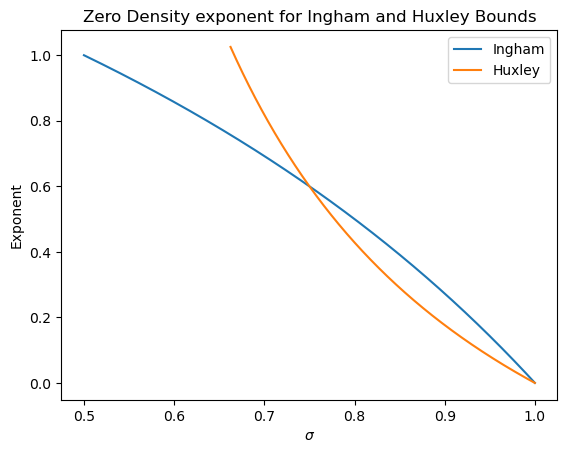
\includegraphics[width=\textwidth]{inghamhuxley1.png}
        \caption{The bounds for the exponent coincide at $\sigma=3/4$}
    \end{subfigure}
    \begin{subfigure}{0.4\textwidth}
        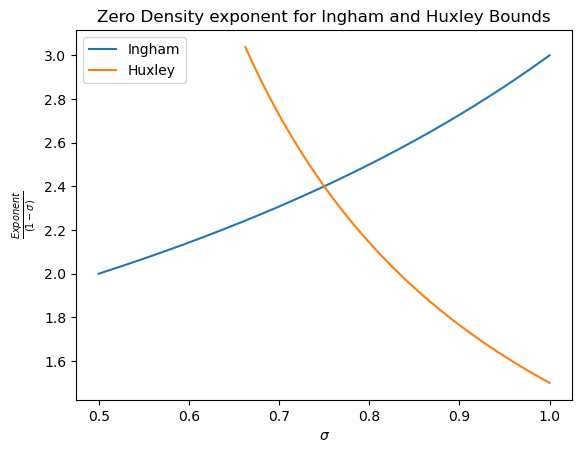
\includegraphics[width=\textwidth]{inghamhuxley2.png}
        \caption{$\sigma=3/4$ is also the bottleneck when written in Hoheisel's form.}
    \end{subfigure}

    \centering
    \begin{subfigure}{0.4\textwidth}
        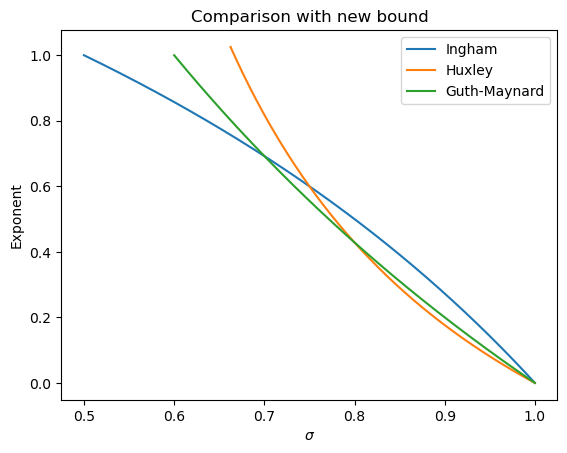
\includegraphics[width=\textwidth]{gm_1.png}
        \caption{Guth-Maynard's result improves in the range at $\sigma\in[7/10,8/10].$}
    \end{subfigure}
    \begin{subfigure}{0.4\textwidth}
        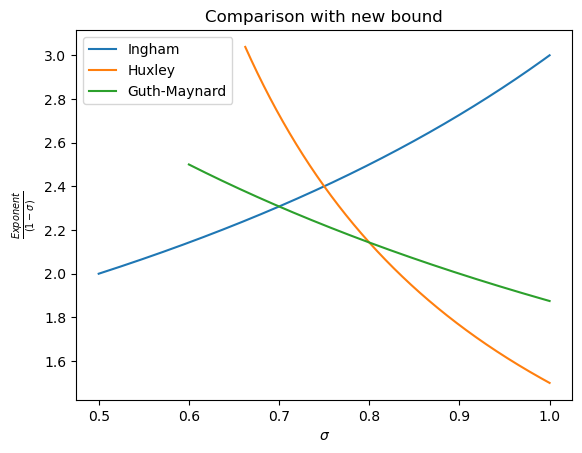
\includegraphics[width=\textwidth]{gm_2.png}
        \caption{The exponent is reduced around the bottleneck region.}
    \end{subfigure}
\end{figure}
	\section{Towards a Hybrid Zero Density Result}
\begin{theorem}[Heath-Brown]
    Let $\mathcal{S}=\{(t_j,\chi_j)\}$ be one-separate, primitive characters of modulus $q$. Then 
    \[
        \sum_{\substack{(t_1,\chi_1)\\(t_2,\chi_2)}}\left|\sum_{n=1}^{N} b_n n^{-i(t_1-t2)}\chi_1\bar{\chi}_2(n)\right|^2 \ll  |\mathcal{S}|N^2+ |\mathcal{S}|^2N + |\mathcal{S}|^{5/4}(qT)^{1/2}N.
    \]
\end{theorem}
\textit{Here I will document some progress with working with
the hybrid version of Guth-Maynard. This section will be removed when I send the draft to Prof. Wunsch.}
Let $\omega$ be a bump function supported on \textit{[placeholder]}. Let $N=T^{[placeholder]}$. We denote \[
D_N(t,\chi) = \sum_{n\sim N} \omega\left(\frac{n}{N}\right)b_n \chi(n) n^{it}
\]
and $\mathcal{S}=\{(t_j,\chi_j)\}_{j\leq |\mathcal{S}|}$ such that 
\[
    |D_N(t_j,\chi_j)|\geq V
\]
for all $(t_j,\chi_j)\in\mathcal{S}$.
We also let $0\leq t_j\leq T$ to be $T^\epsilon$ separated, so if 
$j\neq k$ and $\chi_j=\chi_k$, $|t_j-t_k|\geq T^\epsilon$. \textcolor{red}{We can also
let $\chi_j$'s be Dirichlet characters modulo $q$ (potentially primitive if we need this hypothesis later).}

Here we write $M$ a $|\mathcal{S}\times N|$ matrix with entries
\[
    M_{t_j,\chi_j,n} = \chi_j(n)n^{it_j}
\]
for $(t_j,\chi_j)\in\mathcal{S}$ and $n\sim N$.
Thus by the same reasoning that $(M\vec{b})_j=D_N(t_j,\chi_j)$,
we want to bound the trace of the matrix \[
\textrm{tr}((M^*M)^3)
\]
which is formalized in section $4$ of Guth and Maynard's proof.
We see that \begin{align*}
    (MM^*)_{t_j,t_k} = \sum_{n\sim N} \omega\left(\frac{n}{N}\right)^2 n^{i(t_k-t_j)}\bar{\chi}_j\chi_k(n),
\end{align*}
so that \begin{align*}
    \textrm{tr}(MM^*) = |\mathcal{S}|\sum_{n\sim N} \omega\left(\frac{n}{N}\right)^2
\end{align*}
and Lemmas 4.1-4.4 (Large values controlled by singular values, bound for singular values in terms of trace,
Principle of non-stationary phase, Hilbert-Schmidt Norm estimate) can be adapted directly from the paper.

For the expansion of the trace (analog to lemma 4.5), 
\begin{align*}
    (M^*M)_{n_1,n_2} = \sum_{(t_j,\chi_j)\in \mathcal{S}} \omega\left(\frac{n_1}{N}\right)\omega\left(\frac{n_2}{N}\right)
    \bar{\chi}_j(n_1)\chi_j(n_2)n_1^{-it_j}n_2^{it_j}
\end{align*}
so that \begin{align*}
    \textrm{tr}((M^*M)^3)=\sum_{\substack{(t_1,\chi_1),\\(t_2,\chi_2),\\(t_3,\chi_3)\in\mathcal{S}}}\sum_{n_1,n_2,n_3\sim N} & 
    \omega\left(\frac{n_1}{N}\right)^2 \left(\frac{n}{N}\right)^{i(t_1-t_3)}\chi_1\bar{\chi}_3(n_1)\\
    \times \ &\omega\left(\frac{n_2}{N}\right)^2 \left(\frac{n}{N}\right)^{i(t_2-t_1)}\chi_2\bar{\chi}_1(n_2)\\
    \times \ &\omega\left(\frac{n_3}{N}\right)^2 \left(\frac{n}{N}\right)^{i(t_3-t_2)}\chi_3\bar{\chi}_2(n_3).
\end{align*}
Let $h_t(u)=\omega(u)^2u^{it}$,
so by applying Poisson summation to the inner sum, we have \begin{align*}
    \textrm{tr}((M^*M)^3)=\sum_{\substack{(t_1,\chi_1),\\(t_2,\chi_2),\\(t_3,\chi_3)\in\mathcal{S}}}
    \frac{N^3}{q^3}\sum_{m\in\mathbb{Z}^3}&\sum_{x\in (\mathbb{Z}/q\mathbb{Z})^3}\chi_1\bar{\chi}_3(x_1)\chi_2\bar{\chi}_1(x_2)\chi_3\bar{\chi}_2(x_3) e\left(\frac{-x\cdot m}{q}\right)\\
    \times \ &\hat{h}_{t_1-t_3}\left(\frac{Nm_1}{q}\right)\hat{h}_{t_2-t_1}\left(\frac{Nm_2}{q}\right)\hat{h}_{t_3-t_2}\left(\frac{Nm_3}{q}\right) 
\end{align*}
Finally, we exchange the 2 outermost integrals. And split the sum over $m$ into four parts (same as Guth Maynard) $S_0+ S_1+S_2+S_3$,
where $S_j$ runs over the values of $m$ with exactly $j$ non-zero entries.
\subsection{$S_0$ bound}
$S_0$ only has one term corresponding to $m=0$. By the principle of non-stationary phase, $\hat{h}_t(0)$ has rapid decay in $t$, so contributes $O(T^{-1000})$ except possibly when $t_1,t_2,t_3$ are not $T^\epsilon$ separated.
Moreover, by the orthogonality of characters, all three terms $\chi_a\bar{\chi}_b$ must be principal to have non-zero contribution,
so this fixes the sum to be across $(t_1,\chi_1)=(t_2,\chi_2)=(t_3,\chi_3)$ to give a $N^3\phi(q)^3|\mathcal{S}|\|\omega\|_{L_2}^6/q^3$ term.
So that \begin{align*}
    \textrm{tr}((M^*M)^3)=\frac{N^3\phi(q)^3}{q^3}|\mathcal{S}|\|\omega\|_{L_2}^6 + \sum_{m\in\mathbb{Z}^3 - \{0\}} I_m + O(T^{-100}),
\end{align*}
where \begin{align*}
    I_m=\frac{N^3}{q^3}\sum_{\substack{(t_1,\chi_1),\\(t_2,\chi_2),\\(t_3,\chi_3)\in\mathcal{S}}} &\sum_{x\in (\mathbb{Z}/q\mathbb{Z})^3}\chi_1\bar{\chi}_3(x_1)\chi_2\bar{\chi}_1(x_2)\chi_3\bar{\chi}_2(x_3) e\left(\frac{-x\cdot m}{q}\right)\\
    \times \ &\hat{h}_{t_1-t_3}\left(\frac{Nm_1}{q}\right)\hat{h}_{t_2-t_1}\left(\frac{Nm_2}{q}\right)\hat{h}_{t_3-t_2}\left(\frac{Nm_3}{q}\right).
\end{align*}
which gives the analogous Lemmas 4.5 and 4.6.
\subsection{$S_1$ bound}
\begin{proposition}
    $S_1=O\epsilon(T^{-10})$.
\end{proposition}
By symmetry, we sum $I_m$ across all $m=(0,0,m_3\neq 0)$ at a cost of a factor of $3$.
We then have \begin{align*}
    I_m=\frac{N^3}{q^3}\sum_{\substack{(t_1,\chi_1),\\(t_2,\chi_2),\\(t_3,\chi_3)\in\mathcal{S}}} &\sum_{x\in (\mathbb{Z}/q\mathbb{Z})^3}\chi_1\bar{\chi}_3(x_1)\chi_2\bar{\chi}_1(x_2)\chi_3\bar{\chi}_2(x_3) e\left(\frac{-x_3 m_3}{q}\right)\\
    \times \ &\hat{h}_{t_1-t_3}\left(0\right)\hat{h}_{t_2-t_1}\left(0\right)\hat{h}_{t_3-t_2}\left(\frac{Nm_3}{q}\right)
\end{align*}
Again by the orthogonality of characters, the only way to get non-zero contribution is when $\chi_1=\chi_2$ and $\chi_2=\chi_3$. So this reduces to\begin{align*}
    I_m&=\frac{N^3}{q^3}\sum_{\substack{(t_1,\chi_1),\\(t_2,\chi_2=\chi_1),\\(t_3,\chi_3=\chi_1)\in\mathcal{S}}} \ \phi(q)^2 \sum_{x_3\in (\mathbb{Z}/q\mathbb{Z})^{\times}}e\left(\frac{-x_3 m_3}{q}\right)\\
   & \quad  \times  \quad {h}_{t_1-t_3}\left(0\right)\hat{h}_{t_2-t_1}\left(0\right)\hat{h}_{t_3-t_2}\left(\frac{Nm_3}{q}\right)\\
   &=\frac{N^3}{q^3}\phi(q)^2 \frac{\phi(q)}{\phi\left(\frac{q}{\gcd(m_3,q)}\right)}\mu\left(\frac{q}{\gcd(m_3,q)}\right) \sum_{\substack{(t_1,\chi_1),\\(t_2,\chi_2=\chi_1),\\(t_3,\chi_3=\chi_1)\in\mathcal{S}}} \hat{h}_{t_1-t_3}\left(0\right)\hat{h}_{t_2-t_1}\left(0\right)\hat{h}_{t_3-t_2}\left(\frac{Nm_3}{q}\right)\\
\end{align*}
if 
So we trivially bound $S_1$ by\begin{align*}
    |S_1|&\ll  \frac{N^3}{q^3} \phi(q)^3 \sum_{m_3\neq 0}\sum_{\substack{(t_1,\chi_1),\\(t_2,\chi_2=\chi_1),\\(t_3,\chi_3=\chi_1)\in\mathcal{S}}}
   \left|\hat{h}_{t_1-t_3}\left(0\right)\hat{h}_{t_2-t_1}\left(0\right)\hat{h}_{t_3-t_2}\left(\frac{Nm_3}{q}\right)\right|\\
\end{align*}
By the quick decay and boundedness of $\hat{h}_t(\xi)$ in both $\xi$ and $t$ (decays in terms of $\langle \xi \rangle^{-A}\langle t \rangle^A $ or $ \langle \xi \rangle^A\langle t \rangle^{-A} $), we can bound the terms when summed across all $|m_3|>qT^{1+\epsilon}/N$. For the remaining terms, $t_1\neq t_2$, $t_1\neq t_3$ can be bounded by $O(T^{-10})$.
Finally, when $t_1=t_2=t_3$ and $|m_3|$ is small, we get decay in terms of $(N/q)^{-100}$. 

The sum over terms $|m_3|>qT^{1+\epsilon}/N$,
\begin{align*}
   & \sum_{|m_3|>qT^{1+\epsilon}/N}\sum_{\substack{(t_1,\chi_1),\\(t_2,\chi_2=\chi_1),\\(t_3,\chi_3=\chi_1)\in\mathcal{S}}} 
   \left|\hat{h}_{t_1-t_3}\left(0\right)\hat{h}_{t_2-t_1}\left(0\right)\hat{h}_{t_3-t_2}\left(\frac{Nm_3}{q}\right)\right|\\
    \ll&_{\epsilon,A}  \sum_{|m_3|>qT^{1+\epsilon}/N}\sum_{\substack{(t_1,\chi_1),\\(t_2,\chi_2=\chi_1),\\(t_3,\chi_3=\chi_1)\in\mathcal{S}}} 
    \left|T^{A}\left(\frac{Nm_3}{q} \right)^{-A}\right|\\
    \ll & |\mathcal{S}|^3 T^{-10}.
\end{align*}
For $|m_3|\leq qT^{1+\epsilon}/N$, we use the same bound for terms $t_1\neq t_2$ or $t_1\neq t_3$ by the $\hat{h}_t(0)$ terms. When $t_1=t_2=t_3$, we use $m_3\neq 0$
to bound \[
    \left|\hat{h}_{t_3-t_2}\left(\frac{Nm_3}{q}\right)\right| \ll \left(\frac{q}{N}\right)^{-100}
\]
since $|\mathcal{S}|\ll T\phi(q)$, we can set $T\gg q$ to get the contribution of $S_1$ to be $O\epsilon(T^{-10})$.
\subsection{$S_2$ bound}
We write by symmetry \begin{align*}
    S_2= 3\frac{N^3}{q^3}\sum_{m_1,m_2\neq 0}\sum_{\substack{(t_1,\chi_1),\\(t_2,\chi_2),\\(t_3,\chi_3)\in\mathcal{S}}} &\sum_{x\in (\mathbb{Z}/q\mathbb{Z})^3}\chi_1\bar{\chi}_3(x_1)\chi_2\bar{\chi}_1(x_2)\chi_3\bar{\chi}_2(x_3) e\left(\frac{-x_1m_1-x_2m_2}{q}\right)\\
    \times \ &\hat{h}_{t_1-t_3}\left(\frac{Nm_1}{q}\right)\hat{h}_{t_2-t_1}\left(\frac{Nm_2}{q}\right)\hat{h}_{t_3-t_2}\left(0\right)
\end{align*}
Removing zero contributions from $\chi_2\neq \chi_3$ by orthogonality,
we have \begin{align*}
    =3\frac{N^3}{q^3} \phi(q) \sum_{m_1,m_2\neq 0}\sum_{\substack{(t_1,\chi_1),\\(t_2,\chi_2),\\(t_3,\chi_3=\chi_2)\in\mathcal{S}}} &\sum_{x_1,x_2 \in \mathbb{Z}/q\mathbb{Z}}\chi_1\bar{\chi}_3(x_1)\chi_2\bar{\chi}_1(x_2) e\left(\frac{-x_1m_1-x_2m_2}{q}\right)\\
    \times \ &\hat{h}_{t_1-t_3}\left(\frac{Nm_1}{q}\right)\hat{h}_{t_2-t_1}\left(\frac{Nm_2}{q}\right)\hat{h}_{t_3-t_2}\left(0\right)
\end{align*}
Here, we can isolate contributions from the terms where $t_2\neq t_3$ (hence since $\chi_2=\chi_3$, are $T^{\epsilon}$ separated) to be $O(T^{-10})$. For the other terms, we can write
\[
    \hat{h}_t(\xi) = \overline{\hat{h}_{-t}(-\xi)}
\]
to get 
\iffalse
$S_2$
\begin{align*}
    = 3\frac{N^3}{q^3} \hat{h}_{0}\left(0\right)\phi(q) \sum_{m_1,m_2\neq 0}\sum_{\substack{(t_1,\chi_1),\\(t_2,\chi_2)\in\mathcal{S}}} &\sum_{x_1,x_2 \in \mathbb{Z}/q\mathbb{Z}}\chi_1\bar{\chi}_2(x_1)\chi_2\bar{\chi}_1(x_2) e\left(\frac{-x_1m_1-x_2m_2}{q}\right)\\
    \times \ &\hat{h}_{t_1-t_2}\left(\frac{Nm_1}{q}\right)\hat{h}_{t_2-t_1}\left(\frac{Nm_2}{q}\right)
\end{align*}
and by 

we can rewrite this to get
\fi
\[
    S_2 = 3\frac{N^3}{q^3} \phi(q) \hat{h}_{0}\left(0\right) \sum_{\substack{(t_1,\chi_1),\\(t_2,\chi_2)\in\mathcal{S}}} \left|\sum_{m\neq 0} \sum_{x \in \mathbb{Z}/q\mathbb{Z}}\chi_1\bar{\chi}_2(x) e\left(\frac{-mx}{q}\right)
     \hat{h}_{t_1-t_2}\left(\frac{Nm}{q}\right)\right|^2 + O(T^{-10}).
\]
By the principle of non-stationary phase we can move the terms where $|t_1-t_2|<T^\epsilon$ into $O(T^{-10})$ by decay in $Nm/q$. \textit{We also used the fact that there are at most $\phi(q)$ characters mod $q$, so the $O(q^2)$ factor is negligible compared to $N^{-100}$}.

For the other terms where $t_1$ and $t_2$ are $T^\epsilon$ separated, we want to apply Heath Brown's theorem.

\ 
\\ \ 
\\
\textit{rough work}\ \\
At the cost of $O_\epsilon(T^{-100})$ we can add in the term $\hat{h}_{t_1-t_2}(0)$ in when $t_1,t_2$ are at $T^\epsilon$ separated. Let $W$ be the Mellin transform of the function $\omega(x)^2$.
\begin{align*}
    &N^{1+it}\sum_{m\in \mathbb{Z}} \sum_{x \mod q}\chi(x) e\left(\frac{-mx}{q}\right)
    \hat{h}_{t}\left(\frac{Nm}{q}\right) \\
    =& \sum_{n} n^{it}\chi(n)\omega\left(\frac{n}{N}\right)^2\\
    =& \frac{1}{2\pi i}\int_{2-i\infty}^{2+i\infty}W(s)N^sL(s-it,\chi) ds\\
    =& \frac{1}{2\pi i}\int_{-1-i\infty}^{-1+i\infty}W(s)N^sL(s-it,\chi) ds + \varepsilon(\chi)\frac{\phi(q)}{q}N^{1+it}W(1+it)
\end{align*}
where $\varepsilon$ detects if $\chi$ is principal or not. The second term arising from the (potential) pole at $1$ decays rapidly in $t>T^\epsilon$.
For the first term, we let $\chi$ be induced by the primitive $\chi^*$ with modulus $r$, so\[
    L(s-it,\chi)=L(s-it,\chi^*)\prod_{p|q} \left(1-\frac{\chi^*(p)}{p^s}\right).
\]
We also let \[
    G(s) =\frac{\tau(\chi^*)}{i^\delta\sqrt{r}}r^{s-1/2}\pi^{1/2-s}\frac{\Gamma(\frac{1-s+\delta}{2})}{\Gamma(\frac{s+\delta}{2})},
\]
so that $L(s-it,\chi^*)(s) = G(s-it)L(1-s+it,\overline{\chi^*})$. The integral becomes
\begin{align*}
   &\frac{1}{2\pi i}\int_{-1-i\infty}^{-1+i\infty}W(s)N^sL(s-it,\chi) ds \\=&\frac{1}{2\pi i}
   \int_{-1-i\infty}^{-1+i\infty}W(s)N^s
    G(s-it) L(1-s+it,\overline{\chi^*}) \prod_{p|q} \left(1-\frac{\chi^*(p)}{p^s}\right)ds\\
    =& \frac{1}{2\pi i}\int_{-1-i\infty}^{-1+i\infty}W(s)N^s
    G(s-it) 
    \left(\sum_{n\leq M}\frac{\overline{\chi^*}(n)}{n^{1-s+it}}+
    \sum_{n> M}\frac{\overline{\chi^*}(n)}{n^{1-s+it}}
   \right) \prod_{p|q} \left(1-\frac{\chi^*(p)}{p^s}\right)ds
\end{align*}
Where $M$ is a parameter to be determined. The summation is convergent as the real part is larger than $1$.
We thus break up the integral into two pieces according to the two summations $I_1+I_2$. Moving the line of integration of $I_1$ to $\Re(s)=1$ and $I_2$ to $\Re(s)=-2k$,
\begin{align*}
        I_1&= \frac{1}{2\pi}\int_{-\infty}^{\infty}W(1+iu)N^{1+iu}G(1+iu-it)\sum_{n\leq M}\overline{\chi^*}(n)n^{-i(u-t)}\prod_{p|q} \left(1-\frac{\chi^*(p)}{p^{1+iu}}\right)du,\\
        I_2&= \frac{1}{2\pi}\int_{-\infty}^{\infty}W(-2k+iu)N^{-2k+iu}G(-2k+iu-it)\sum_{n> M}\overline{\chi^*}(n)n^{-2k-1-i(u-t)}\prod_{p|q} \left(1-\frac{\chi^*(p)}{p^{-2k+iu}}\right)du.
\end{align*}
By the decay of $W$, we can truncate both integrals to the region $|u|\ll T^\epsilon$.
Moreover, \textit{decay of gamma - might have a typo in GM paper?}
\section{$S_3$ bound}
By non-stationary phase, $I_m$ is negligible for the terms $qT/N\lesssim |m|$, so 
\begin{equation}
    S_3 = \sum_{0<|m_1|,|m_2|,|m_3|\lesssim qT/N} I_m + O(T^{-100}).
\end{equation}
We define \begin{align*}
    R(v,n_1,n_2)&\defeq \sum_{(t,\chi)\in \mathbb{S}} 
    \chi({n_1})\bar{\chi}(n_2)v^{it},\\
    R(v,n)&\defeq R(v,n,1).
\end{align*}
\begin{proposition}
    \[
    |I_m|\ll \phi(q) \frac{N^3}{q^3}  
    \sum_{y_1,y_2\in (\mathbb{Z}/q\mathbb{Z})^\times}\ \int\displaylimits_{\substack{
        |v_1m_1+v_2m_2+m_3|\lesssim \frac{q}{N}\\
        \frac{1}{2}\leq v_1,v_2\leq 2
    }} \left| R\left(\frac{v_1}{v_2},y_1,y_2\right)
    R(v_2,y_2)R\left(v_1,y_1\right)\right| dv_1 \ dv_2  + O(T^{-100}).\\
    \]
    Moreover, if $|m_1|\leq|m_2|\leq |m_3|$, $|I_m|=O(T^{-100})$ unless $|m_2|\asymp|m_3|$.
\end{proposition}
\begin{proof}
    
Recall
\begin{align*}
    I_m=\frac{N^3}{q^3}\sum_{\substack{(t_1,\chi_1),\\(t_2,\chi_2),\\(t_3,\chi_3)\in\mathcal{S}}} &\sum_{x\in (\mathbb{Z}/q\mathbb{Z})^3}\chi_1\bar{\chi}_3(x_1)\chi_2\bar{\chi}_1(x_2)\chi_3\bar{\chi}_2(x_3) e\left(\frac{-x\cdot m}{q}\right)\\
    \times \ &\hat{h}_{t_1-t_3}\left(\frac{Nm_1}{q}\right)\hat{h}_{t_2-t_1}\left(\frac{Nm_2}{q}\right)\hat{h}_{t_3-t_2}\left(\frac{Nm_3}{q}\right).
\end{align*}
Expanding the integrals, 
\begin{align*}
    I_m=\frac{N^3}{q^3}\sum_{\substack{(t_1,\chi_1),\\(t_2,\chi_2),\\(t_3,\chi_3)\in\mathcal{S}}} &\sum_{x\in (\mathbb{Z}/q\mathbb{Z})^3}\chi_1\bar{\chi}_3(x_1)\chi_2\bar{\chi}_1(x_2)\chi_3\bar{\chi}_2(x_3) e\left(\frac{-x\cdot m}{q}\right)\\
    \times \ &
    \int_{\reals^3}\mathbf{\tilde{\omega}}(\mathbf{u})u_1^{i(t_1-t_3)}u_2^{i(t_2-t_1)}u_3^{i(t_3-t_2)}e\left(\frac{-N\mathbf{m}\cdot \mathbf{u}}{q}\right)d\mathbf{u},
\end{align*}
where $\tilde{\omega}(\mathbf{u})=\omega(u_1)^2\omega(u_2)^2\omega(u_3)^2$ is compactly supported.
We now make the substitution $y_1=x_1x_3^{-1}, y_2=x_2x_3^-1 \mod q$ for the summation over $x$, and $v_1=u_1/u_3,v_2=u_2/u_3$ for the integral on the support of $\tilde{\omega}$.
We thus rewrite the sum over $x$ as 
\begin{align*}
    &\sum_{y_1,y_2,x_3\in (\mathbb{Z}/q\mathbb{Z})^\times}
    \chi_1(y_1y_2^{-1})\chi_2(y_2)\chi_3(y_1^{-1})e\left(\frac{-(y_1m_1+y_2m_2+m_3)x_3}{q}\right)\\
    =&
    \sum_{y_1,y_2\in (\mathbb{Z}/q\mathbb{Z})^\times}\chi_1(y_1)\bar{\chi}_1(y_2)\chi_2(y_)\bar{\chi}_3(y_1)\sum_{x_3\in (\mathbb{Z}/q\mathbb{Z})^\times}e\left(\frac{-(y_1m_1+y_2m_2+m_3)x_3}{q}\right),
\end{align*}
where we can use the trivial bound $\phi(q)$ for the innermost sum.
We also rewrite triple integral as 
\begin{align*}
    &\int_{\reals^3}\tilde{\omega}(v_1u_3,v_2u_3,u_3) {\left(\frac{v_1}{v_2}\right)}^{it_1} {\left(v_2\right)}^{it_2}{\left(\frac{1}{v_1}\right)}^{it_3} u_3^2 \ e\left(\frac{-N(v_1m_1+v_2m_2+m_3)u_3}{q}\right)\ dv_1\ dv_2\ du_3\\
    =&\int_{\reals^2}\int_\reals u_3^2 \ \tilde{\omega}(v_1u_3,v_2u_3,u_3) e\left(\frac{-N(v_1m_1+v_2m_2+m_3)u_3}{q}\right)  du_3 \ {\left(\frac{v_1}{v_2}\right)}^{it_1} {\left(v_2\right)}^{it_2}{\left(\frac{1}{v_1}\right)}^{it_3}  \ dv_1\ dv_2.\\
\end{align*}
The integrand of the innermost integral is non-zero only if \[
    v_1u_3,v_2u_3,u_3\sim N.
\]
Importantly, this requires $1/2 \leq v_1,v_2 \leq 2$, so we can truncate the outermost integrals to these regions. Moreover, by repeated integration by parts, this integral is $O_{\epsilon, A}(T^{-A})$ for any $|v_1m_1+v_2m_2+m_3|>qT^\epsilon/N$.
So 
\begin{align*}
    |I_m|\ll &\phi(q) \frac{N^3}{q^3}  
    \sum_{y_1,y_2\in (\mathbb{Z}/q\mathbb{Z})^\times}\left|\ \int\displaylimits_{\substack{
        |v_1m_1+v_2m_2+m_3|\lesssim \frac{q}{N}\\
        \frac{1}{2}\leq v_1,v_2\leq 2
    }} R\left(\frac{v_1}{v_2},y_1,y_2\right)
    R(v_2,y_2)R\left(\frac{1}{v_1},1,y_1\right) dv_1 \ dv_2 \right|\\ &+ O(T^{-100}).\\
\end{align*}
Since $|R(v_1^{-1},1,y_1)|=|R(v_1,y_1)|$, we have the first part of the proposition.
The second part of the proposition follows from the integral bounds $|v_1m_1+v_2m_2+m_3|\lesssim q/N$
 and $v_1,v_2\asymp 1$. These force $|m_2| \asymp|m_3|$, or else the integral will be zero.

\end{proof}

Adapting from Guth and Maynard, when $|m_2|\asymp|m_3|$, the domain of integration can be written as\begin{align*}
    |v_1m_1+v_2m_2+m_3|\lesssim \frac{q}{N} \implies \left|v_2 - \frac{v_1m_1+m_3}{-m_2}\right|\lesssim \frac{q}{|m_2|N} \asymp \frac{q}{|m_3|N}.
\end{align*}
Thus, 


\textcolor{red}{TODO}
\begin{proposition}
    There is a choice of $0<M_1\leq M \lesssim qT/N$ such that \[
        S_3\lesssim \phi(q)\frac{N^2}{M}\sum_{|m_1|\sim M_1,|m_2|,|m_3|\sim M}\tilde{I}_m+O(T^{-100}).
    \]
    where \[
    \tilde{I}_m\defeq \sum_{y_1,y_2\in (\mathbb{Z}/q\mathbb{Z})^\times}\ \int_{v_1\asymp 1} 
         \left|R\left(v_1,y_1\right) \tilde{R}_M\left(\frac{m_1v_1+m_3}{-m_2v_1},y_2,y_1\right)
        \tilde{R}_M(\frac{m_1v_1+m_3}{-m_2},y_2)\right| dv_1.
    \]
\end{proposition}


\begin{proof}
    \textcolor{red}{TODO}
\end{proof}


\begin{lemma} \label{secondmoment}
    Let $\mathbb{S}=\{(t_j,\chi_j)\}$, and the $t$'s are contained in an interval of length $T$, and are $T^\epsilon$-separated for the same character. Then \[
        \sum_{y\in (\mathbb{Z}/q\mathbb{Z})^\times} \int_{v\asymp 1} 
        \left|R\left(v,y\right)\right|^2dv \ll_{\epsilon} \phi(q)|\mathbb{S}|.
    \]
\end{lemma}
\begin{proof}
    We have \[
    |R(v,y)|^2 = \sum_{(t_1,\chi_1),(t_2,\chi_2)\in \mathbb{S}}
    \chi_1\bar{\chi}_2(y)v^{i(t_1-t_2)}.
    \]
    Let $\psi$ be a bump function supported on $v\asymp 1$ and equals $1$ on the domain of integration in the lemma.
    By orthogonality of characters, \begin{align*}
        \sum_{y\in (\mathbb{Z}/q\mathbb{Z})^\times} \int_{v\asymp 1} 
        \left|R\left(v,y\right)\right|^2dv 
        \leq&\sum_{y\in (\mathbb{Z}/q\mathbb{Z})^\times} \int 
        \psi(v)\left|R\left(v,y\right)\right|^2dv 
        \\=&
        \phi(q)\int \psi(v)
        \sum_{\substack{(t_1,\chi_1),(t_2,\chi_2)\in \mathbb{S}\\ \chi_1=\chi_2}}v^{i(t_1-t_2)}
        dv\\
        =&
        \phi(q)\sum_{\substack{(t_1,\chi_1),(t_2,\chi_2)\in \mathbb{S}\\ \chi_1=\chi_2}}\int \psi(v)
        v^{i(t_1-t_2)}
        dv.
    \end{align*}
    In the sum, the terms $t_1=t_2$ contribute $O(|\mathbb{S}|)$. If $t_1\neq t_2$, then $|t_1-t_2|\geq T^\epsilon$. The integral in this case is $O_\epsilon(T^-100)$ and is negligible.
\end{proof}
\begin{lemma}\label{fourthmoment}
    Let $E(\mathbb{S})=\#\{(t_1,\chi_1),(t_2,\chi_2),(t_3,\chi_3),(t_4,\chi_4)\in \mathbb{S}  :  |t_1+t_2-t_3-t_4|\leq 1, \chi_1\chi_2=\chi_3\chi_4\}$. Then \[
        \sum_{y\in (\mathbb{Z}/q\mathbb{Z})^\times} \int_{v\asymp 1} 
        \left|R\left(v,y\right)\right|^4dv  \lesssim \phi(q)E(\mathbb{S}).
    \]
\end{lemma}
\begin{proof}
    We have \[
    |R(v,y)|^4 = \sum_{\substack{(t_1,\chi_1),(t_2,\chi_2),\\ (t_3,\chi_3),(t_4,\chi_4)\in \mathbb{S}}}
    \chi_1{\chi}_2\bar{\chi_3}\bar{\chi_4}(y)v^{i(t_1+t_2-t_3-t_4)}.
    \]
    So again by the orthogonality of characters, \begin{align*}
        \sum_{y\in (\mathbb{Z}/q\mathbb{Z})^\times} \int_{v\asymp 1} 
        \left|R\left(v,y\right)\right|^4dv = & \phi(q)
        \sum_{\substack{(t_1,\chi_1),(t_2,\chi_2),\\ (t_3,\chi_3),(t_4,\chi_4)\in \mathbb{S}\\ \chi_1\chi_2=\chi_3\chi_4}} \int_{v\asymp 1} v^{i(t_1+t_2-t_3-t_4)} dv.
    \end{align*}
    Similar to the previous proof, we can introduce a bump function for the integral, and restrict the summation to the terms $|t_1+t_2-t_3-t_4|\leq T^\epsilon$ with an error of $O_\epsilon(T^{-100})$. The remaining terms in the summation contribute $O(E(\mathbb{S}))$.
\end{proof}
\begin{proof}[{Proof of proposition [placeholder]}]
    We first appler H\"older's inequality on the integral to get 
    \begin{align*}
        \tilde{I}_m \leq  \sum_{y_1,y_2\in (\mathbb{Z}/q\mathbb{Z})^\times}& \left(\int_{v_1\asymp 1} 
        \left|R\left(v_1,y_1\right)\right|^2dv_1\right)^{1/2} \left(\int_{v_1\asymp 1} \left|\tilde{R}_M\left(\frac{m_1v_1+m_3}{-m_2v_1},y_2,y_1\right)\right|^4 dv_1\right)^{1/4} \\& \left(\int_{v_1\asymp 1} 
       \left| \tilde{R}_M(\frac{m_1v_1+m_3}{-m_2},y_2)\right|^{4} dv_1\right)^{1/4},
    \end{align*}
    Notice the first integral is independent of $y_2$, for sum of the second and third integrals over $y_2$, we apply Cauchy-Schwarz to get\begin{align*}
        &\sum_{y_2\in (\mathbb{Z}/q\mathbb{Z})^\times}\left(\int_{v_1\asymp 1} \left|\tilde{R}_M\left(\frac{m_1v_1+m_3}{-m_2v_1},y_2,y_1\right)\right|^4 dv_1\right)^{1/4} \left(\int_{v_1\asymp 1} 
       \left| \tilde{R}_M(\frac{m_1v_1+m_3}{-m_2},y_2)\right|^{4} dv_1\right)^{1/4}\\
       \leq& \left(\sum_{y_2\in (\mathbb{Z}/q\mathbb{Z})^\times}\left(\int_{v_1\asymp 1} \left|\tilde{R}_M\left(\frac{m_1v_1+m_3}{-m_2v_1},y_2,y_1\right)\right|^4 dv_1\right)^{1/2}\right)^{1/2}\\ &\quad \quad
       \left(
       \sum_{y_2\in (\mathbb{Z}/q\mathbb{Z})^\times} \left(\int_{v_1\asymp 1}
       \left| \tilde{R}_M(\frac{m_1v_1+m_3}{-m_2},y_2)\right|^{4} dv_1 \right)^{1/2}\right)^{1/2}
       \\ 
       \leq&  \phi(q)^{\frac{1}{2}} \left(\sum_{y_2\in (\mathbb{Z}/q\mathbb{Z})^\times}\int_{v_1\asymp 1} \left|\tilde{R}_M\left(\frac{m_1v_1+m_3}{-m_2v_1},y_2,y_1\right)\right|^4 dv_1\right)^{1/4}\\ &\quad \quad
       \left(
       \sum_{y_2\in (\mathbb{Z}/q\mathbb{Z})^\times} \int_{v_1\asymp 1}
       \left| \tilde{R}_M(\frac{m_1v_1+m_3}{-m_2},y_2)\right|^{4} dv_1\right)^{1/4} \\
       \leq&  \phi(q)^{\frac{1}{2}} \left(\sum_{y_3\in (\mathbb{Z}/q\mathbb{Z})^\times}\int_{v_1\asymp 1} \left|\tilde{R}_M\left(\frac{m_1v_1+m_3}{-m_2v_1},y_3\right)\right|^4 dv_1\right)^{1/4}\\ &\quad \quad
       \left(
       \sum_{y_2\in (\mathbb{Z}/q\mathbb{Z})^\times} \int_{v_1\asymp 1}
       \left| \tilde{R}_M(\frac{m_1v_1+m_3}{-m_2},y_2)\right|^{4} dv_1\right)^{1/4}
       \\ \lesssim&
       \phi(q)E(\mathbb{S})^{\frac{1}{2}}(M/M_1)^{1/4}\leq\phi(q)E(\mathbb{S})^{\frac{1}{2}}M/M_1.
       \end{align*}
       where in the penultimate step, we made a change of variables $y_3=y_2y_1^{-1}$. In the last step we change variables of integration $u=(m_1v_1+m_3)/(-m_2v_1)$ and $u=(m_1v_1+m_3)/(-m_2)$ with a Jacobian factor of $\asymp 1$ and $\sim M/M_1$ respectively. 
       For the first integral, applying Cauchy Schwarz gives \begin{align*}
        \sum_{y_1\in (\mathbb{Z}/q\mathbb{Z})^\times} \left(\int_{v_1\asymp 1} 
        \left|R\left(v_1,y_1\right)\right|^2dv_1\right)^{1/2} 
        \leq  \phi(q)^{\frac{1}{2}}\left(\sum_{y_1\in (\mathbb{Z}/q\mathbb{Z})^\times} \int_{v_1\asymp 1} 
        \left|R\left(v_1,y_1\right)\right|^2dv_1\right)^{1/2} 
        \ll_{\epsilon} |\mathbb{S}|.
       \end{align*}
       Combined, this gives \[
       S_3 \leq 
       \]
\end{proof}

\section{Energy bound}
Here we provide the generalization for the orthogonal energy bound for Guth and Maynard's result. 

The idea for bounding energy is similar, if $\chi_1\chi_2=\chi_3\chi_4$ and $|t_1+t_2-t_3-t_4|$ is small, we should expect $|D_N(t_1+t_2-t_3,\chi_1\chi_2\bar{\chi}_3)|\simeq |D_N(t_4,\chi_4)|>N^\sigma$.
\begin{lemma}
    \[
    D_N(t,\chi)\lesssim \int_{|u-t|\lesssim 1} |D_N(u,\chi)|du + O(T^{-100}).
    \]
\end{lemma}
\begin{proof}
    \begin{align*}
        D_N(t,\chi)=\sum_n \omega\left(\frac{n}{N}\right) b_n n^{it} \psi\left(\frac{\log n}{2\pi}\right)
    \end{align*}
\end{proof}
	\section*{Preliminaries}
Here we provide some supplementary definitions and statements of theorems. These results are well-known. 
\subsection*{Number Theory}
\begin{definition}[Dirichlet Characters]
	\label{dcharacter}
	Let $q\in\naturals$. A Dirichlet character $\chi:\mathbb{N}\to\complex$ modulus $q$ is an arithmetic function satisfying \begin{itemize}
		\item \textit{(Periodicity)} $\chi(n+q)=\chi(n)\forall n\in\naturals$.
		\item \textit{(Complete multiplicativity)} $\chi(nm)=\chi(n)\chi(m)\forall n,m\in\naturals$.
		\item $|\chi(n)|=\begin{cases}
			1, & \rm{if }\gcd(n,q)=1,\\
			0, & \rm{otherwise.}
		\end{cases}$
	\end{itemize}
\end{definition}
\begin{proposition}
	There are $\phi(q)$ Dirichlet characters of modulus $q$.
\end{proposition}
\begin{proof}
	Taking residual classes mod $q$, we see that Dirchlet characters are in one-to-one correspondence with one-dimensional representations of the multiplicative group $(\mathbb{Z}/q\mathbb{Z})^{\times}$. Since this group is abelian, all of its irreducible representations are one-dimensional. Therefore, the number of Dirichlet characters equals the number of irreducible representations of the $(\mathbb{Z}/q\mathbb{Z})^{\times}$. It is known that the sum of squares of the dimensions irreducible representations equals the order of the group, so we have \[
		\phi(q)=|(\mathbb{Z}/q\mathbb{Z})^{\times}|=\sum_{\textrm{irreducible representations } \varphi}  (\textrm{dim } \varphi)^2 = \sum_{\textrm{irreducible representations } \varphi}  1.
	\]
\end{proof}
\begin{definition}
	A Dirichlet character $\chi$ modulus $q$ is induced by another character $\chi^*$ mod $m<q$ if they agree on all $n$ such that $\gcd(q,n)=1$. A Dirchlet character is primitive if it is not induced by another character. A Dirchlet character is principal if it is induced by the character $\chi_1(n)\defeq1(n)\equiv 1$, thus corresponds to the trivial representation.
\end{definition}
\begin{theorem}[M\"obius Inversion]
	The M\"obius function $\mu$ is defined for $n\in\naturals$,
	\[
		\mu(n) = \begin{cases}
			1, \textrm{ if } n=1\\
			(-1)^k, \textrm{ if }n=p_1p_2...p_k\textrm{ for distinct }p\textrm{'s}\\
			0, \textrm {otherwise}
		\end{cases}
	\]
	Suppose we have arithmetic functions $f,g$, and that\[
		f(n) = \sum_{d|n} g(d)
	\]
	Then the M\"obius Inversion formula gives 
	\[
		g(n) = \sum_{d|n} \mu(d) f\left(\frac{n}{d}\right)
	\]
\end{theorem}
\begin{example}
	On $\Re(s)>1$, let $M_N(s) = \sum_{n\leq N} \mu(n)n^{-s}$.
	Then setting $f(n)=1$ for all $n$, $g(1)=1$, $g(n)=0$ for $n\geq 2$, we multiply $M_N$ by $\zeta$ in Dirichlet series to get\[
		\zeta(s)M_N(s) = \sum_{n} \frac{a_n}{n^{-s}},
	\]
	where $a_n=g(n)$ for all $n\leq N$.
	Similarly, letting $M_N(s) = \sum_{n\leq N} \chi(n) \mu(n) n^{-s}$ for some Dirichlet character $\chi$,
	we get \[
		L(s,\chi)M_N(s) = \sum_{n} \frac{a_n\chi(n)}{n^{-s}}
	\]
	with the same $a_n$ as in the previous equation.
\end{example}
\begin{theorem}[Erd\"os-Kac]
	Let $\omega(n)$ be the number of prime divisors of $n$, ignoring multiplicity. Let $X_N\sim \rm{unif}\{1,N\}$, the uniform distribution from $1$ to $N$, and
	\[
	Y_N\defeq \frac{\omega(X_N)-\log\log X_N}{\sqrt{\log \log X_N}}.
	\] 
	Then \[
	\lim_{N\to\infty} P(a<Y_N<b) = \frac{1}{\sqrt{2\pi}}\int_a^b e^{-t^2/2}dt.
	\]
\end{theorem}
\subsection*{Harmonic Analysis}
\begin{theorem}[Fourier Inversion]
	In Schwartz space, the Fourier transform of $\mathcal{F}:\schwartz(\reals^d)\to\schwartz(\reals^d)$ of $f\in\mathcal{S}(\reals^d)$ is given by
    \[
        \hat{f}(\mathbf{\xi})\defeq\mathcal{F}f(\mathbf{\xi})\defeq \int_{\reals^d} e(- \mathbf{\xi}\cdot \mathbf{x}) f(\mathbf{x}) \ d\mathbf{x}
    \]
    has inverse given by 
    \[
       f(\mathbf{x})= \mathcal{F}^{-1}\hat{f}(\mathbf{x})\defeq \int_{\reals^d} e(\mathbf{\xi}\cdot \mathbf{x}) \hat{f}(\mathbf{\xi}) \ d\mathbf{\xi}.
    \]
\end{theorem}
\begin{theorem}[Discrete Fourier Inversion]
	Let $g$ be an arithmetic function that is periodic$\mod q$. We define the discrete Fourier transform of $g$ to be \[
		\hat{g}(y) \defeq \sum_{x \mod q}g(x)e\big(-\frac{xy}{q}\big)
	\]
	which is periodic $\mod q$.
	This has inverse given by \[
		g(x) = \frac{1}{q}\sum_{y\mod q} \hat{g}(y)e\big(\frac{xy}{q}\big).
	\]
\end{theorem}
\begin{theorem}[Plancherel/Parsavel]
We have \[
\|f\|_{L^2}=\|\hat{f}\|_{L^2}
\]
for Schwartz functions and \[
\sum_{x\mod q}|g(x)|^2 = \frac{1}{q}\sum_{y\mod q}|\hat{g}(y)|^2
\]
for the discrete Fourier transform of functions periodic$\mod q$.

\end{theorem}
\begin{theorem}[Mellin Inversion]
	The Mellin transform of a function $f:(0,\infty)\to\complex$
	\[
	\tilde{f}(s) \defeq \mathcal{M}f(s) \defeq \int_{0}^{\infty}f(x) x^{s-1} \ dx
	\]
	has inverse \[
	\mathcal{M}^{-1} \tilde{f} (x) = \int_{c-i\infty}^{c+i\infty} \tilde{f}(s) x^{-s}ds
	\]
	on $a<c<b$ provided that the integral $\tilde{f}$ is absolute convergent on the strip $a<\Re(s)<b$.
\end{theorem}
\begin{theorem}[Poisson Summation]
	Let $f:\reals\to\complex$ be Schwartz. Then \[
	\sum_{n\in \mathbb{Z}} f(n) = \sum_{\xi\in\mathbb{Z}} \hat{f}(\xi).
	\]
\end{theorem}
\end{document} 